\pagebreak
\section{ПРОГРАММА И МЕТОДИКА ИСПЫТАНИЙ}
\label{sec:testing}

В данном разделе будет рассмотрено тестирование разработанного программного обеспечения.

Так как данный продукт представляет из себя систему компонентов, которая использует полноценный кластер, то и тестирование будет производиться в двух напрвлениях:
\begin{itemize}
    \item юнит-тестирование;
    \item интеграционное тестирование.
\end{itemize}

Большое внимание будет уделяться именно интеграционному тестированию, так как оно позволяет проверить рабатоспособность всей системы.
Можно сказать, что такое тестирование определяет наличие ошибки в приложении.
Юнит-тестирование в свою очередь помогает определить, в каком именно модуле произошла ошибка.

Важность тестирования возрастает и с тем, что проект является открытым, и поэтому обязательно необходимо тестировать все изменения.
Также для удобства тестирования были использованы инструменты для непрерывной интеграции.
В частности для непрерывной интеграции использовались:
\begin{itemize}
    \item Jenkins;
    \item Gitlab - pipelines.
\end{itemize}


Jenkins представляет из себя Java веб приложение, которое запускается на хосте, и позволяет запускать команды на этом хосте.
Таким образом, с помощью файла \texttt{./Jenkinsfile} идёт описание инструкций, которые необходимо выполнить для репозитория на используемой машине.
Более подробно с Jankins можно ознакомится на сайте с его документацией~\cite{jenkins_documentation}.

Таким образом, если на используемом хосте установлен Docker, то это позволяет полностью развернуть всю необходимую инфраструктуру для запуска всей системы.
Также есть возможность настроить Jenkins на проверку удалённого репозитория по расписанию.
Если с момента последнего запуска, в удалённый репозиторий были закоммичены изменения, то как только jenkins проверит удалённый репозиторий - он выполнит команды, которые указаны в репозитории.
Такой режим работы называется трубой (англ. pipeline).
Также можно запускать команды и вручную.

Аналогичным инструментом является Gitlab - pipelines.
Благодаря возможности интеграции с сервисом Github - такой инструмент позволяет запускать 

\subsection{Интеграционное тестирование}

Для запуска тестов необходимо запустить скрипт \texttt{test.sh}.
С помощью данного скрипта вызывается докер, в котором разворачивается вся необходимая инфраструктура, а также и разработанные компоненты системы.
В качестве интеграционного теста происходит проверка отправки и получения сообщений, которые передаются с помощью kafka.

С помощью докера запускаются следующие компоненты:
\begin{itemize}
    \item zookeeper;
    \item kafka;
    \item отправитель.
\end{itemize}

Отправитель использует настройки для тестирования.
Однако, для взаимодействия со внешним сервисом необходим ключ, что уже было отмечено раньше.
По этой причине, ключ передаётся в качестве аргумента при запуске скрипта \texttt{test.sh}.
Скрипт подменяет значение по-умолчанию в файле конфигурации.
Таким образом, появляется возможность запускать интеграционные тесты с помощью скрипта.

Также, при использовании средств непрерывной интеграции появляется возможность задать такой ключ прямо в настройках пайплайна.
По этой причине, в качестве аргумента для скрипта \texttt{test.sh} в jenkinsfile используется переменная окружения:
\begin{lstlisting}
    sh "./test.sh --api-key ${OPEN_WEATHER_MAP_API_KEY}"
\end{lstlisting}

Данное значение устанавливается в самих настройках пайплайна в jenkins.
Такой подход позволяет скрыть действительно используемый API ключ от других участников проекта.
В свою очередь каждый участник сможет использовать свой собственный ключ для тестирования, либо для использования проекта.

После того, как все компоненты были запущены, отправитель перебирает установленный диапазон параметров, и пытается получить для них данные.
Всё действует точно также, как и при настоящей работе программы: сначала происходит проверка локального хранилища, а в случае отсутствия данных - происходит обращение к внешнему сервису.
Все отправленные сообщения отправляются в топик для тестирования.
Это позволяет при желании использовать тот же kafka брокер, который будет использоваться и при работе программы.
В таком случае, происходит тестирование продукта в <<полевых>> условиях.

После того, как сообщения были отправлены в брокер, отдельный получатель проверяет количество сообщений в тестовом топике.
Количество сообщений должно совпадать с диапазоном значений, который был использован при отправлении значений.
Если же количество сообщений не совпадает - значит какие-то данные не были отправлены в топик.
Это означает, что такая система не может полноценно работать, поэтому использование текущего окружения и настроек приведёт к ошибочному поведению программы.

Такое тестирование позволяет уловить само наличие ошибок, однако не предоставляет точной информации, в какой именно части произошёл сбой.
Поэтому, при тестировании ведётся логгирование программы, что позволяет отследить полный ход программы.
Возможные причины отсутствия сообщений:
\begin{itemize}
    \item недоступность kafka-брокера;
    \item используемый топик не был создан;
    \item был указан неверный путь к локальному хранилищу;
    \item был указан неверный API-ключ;
    \item используемый API-ключ не имеет необходимой подписки для использования API для получения индекса загрязнений;
    \item отсутствие связи с сервером;
    \item неработоспособность zookeeper сервера;
    \item используемый порт уже используется другим приложением;
    \item недоступный удалённый адрес распределённой системы при использовании таковой;
    \item системные ошибки.
\end{itemize}

К системным ошибкам относятся недостаток свободного места на диске, нехватка оперативной памяти, принудительное завершение процесса и тому подобное.
Остальные ошибки можно распознать при чтении log-файла.


\subsection{Юнит тестирование}
Юнит тестирование выполняет функцию локализации ошибки.
Другими словами, при установке наличия ошибки, с помощью юнит тестов можно определить, в какой чатси программы она произошла.
Также юнит тестирование применяется для проверки работоспособности модуля, что позволяет проверять внесённые изменения в отдельный компонент программы, без запуска всей системы.

Для юнит тестирования использовалась библиотека \texttt{pytest}.
Компоненты программы, которые подвергаются тестированию:
\begin{itemize}
    \item классы для обработки конфигурации;
    \item классы для работы с файловой системой;
    \item классы для получения данных из внешнего сервиса;
    \item классы для преобразовния данных;
    \item классы для подключения и отправки сообщений.
\end{itemize}

\subsubsection{Тестирование классов конфигурации}

Главная задача классов конфигурации - правильно обработать исходный файл конфигурации и на его основе создать параметры конфигурации для всего приложения.
В качестве параметров используется список строк, что позволяет проводить тестирование данных классов без использования файлов конфигурации.
При тестировании создаётся список строк, каждая из которых определяет параметр.
В результате такой обработки, параметры, которые были переданы, и параметры, которые содержатся в созданном экземпляре класса должны быть идентичными.

Один из примеров тестирования обработки конфигурации:
\begin{lstlisting}
def test_fs_parse_from_lines(self):
    lines = [
        "Dir   :  /users/hdfs/dumper/test_out/ ",
        "Host : 10.0.2.5:8088"
    ]
    actual = FSConfig.parse_from_lines(lines)
    expected = FSConfig("/users/hdfs/dumper/test_out/", "10.0.2.5:8088")
    self.assertEqual(actual, expected, "FS Configs are not equal")
\end{lstlisting}

\subsubsection{Тестирование классов работы с файловой системой}

Главная задача классов для работы с файловой системой - производить простые операции с файловой системой.
В частности, такие операции как:
\begin{itemize}
    \item запись в файл;
    \item чтение из файла;
    \item создание директории;
    \item удаление файла;
    \item получение списка файлов в директории;
    \item проверка существования файла.
\end{itemize}

Для тестирования этих операций, создаётся директория, которая предназначена для тестирования.
В этой директории как раз и будут создаваться и удаляться файлы в ходе тестирования.
Для тестирования записи в файл - происходит запись в файл определённых данных, а после происходит вычитывание данных из созданного файла.
При идентичности записанных и считанных данных тест считается пройденным.
Для проверки чтения всё происходит аналогично, только в этот раз чтение осуществляется с помощью тестируемого класса, а запись - при помощи стандартных средств.

При проверке удаления файла, сначала происходит получение файлов в тестовой директории.
После этого происходит удаление одного файла.
Далее снова происходит получение списка файлов в тестовой директории.
После происходит сравнение списка до удаления и после.

\subsubsection{Тестирование классов для получения данных}

Главная задача классов для получения данных является обращение к внешнему сервису и отправка запроса к нему.
Тестированию подвергается два аспекта данных классов:
\begin{itemize}
    \item построение запроса к внешнему сервису;
    \item сохранение и выдача результата при успешном запросе.
\end{itemize}

Для тестирования построения запроса к внешнему сервису происходит конфигурирование класса для запроса и вызов метода построения URL адреса.
Полученный адрес сравнивается с ожидаемым адресом для используемых аргументов.
Пример такого тестирования для одного из запросов:

\begin{lstlisting}
def test_co_address(self):
    co_dumper = CODumper("some_host", "atztpcnk", "test", self.__adapter)
    actual = co_dumper.to_address(25, 45, 2017)
    expected = "some_host/co/25,45/2017.json?appid=atztpcnk"
    self.assertEqual(actual, expected)
\end{lstlisting}

Для тестирования сохранения и выдачи данных происходит подмена функции запроса.
При нормальной работе класс использует стандартную функцию для отправки запроса.
Однако если использовать такой вариант при тестировании - появляется зависимость от внешних факторов, таких как подключение устройства к внешней сети, работоспособность внешнего сервиса и корректность используемого ключа.
Так как тестирование должно быть максимально изолированным и не должно зависеть от внешних факторов, то добавляется возможность подменить используемую функцию для отправки запроса на любую другую.
Такой подход позволяет протестировать саму логику приложения.

В итоге происходит подмена функции отправки запроса на ложную.
Например, одна из таких функций:
\begin{lstlisting}
def mock_oz_request(address):
    if address == "some_host/o3/24,92/2018.json?appid=atztpcnk":
        return ResponseMock(200, "Yes, it's ok")
    return ResponseMock(400, "Something wrong")
\end{lstlisting}

\subsubsection{Тестирование классов обработки данных}

Главная цель классов обработки данных является преобразование полученных данных в формате JSON в вид, который позволяет легко их обрабатывать.
При тестировании таких классов происходит обработка заготовленного JSON объекта и проверяется результат обработки.
При идентичности полученного и ожидаемого результата тест считается успешным.

Результаты тестирования представлены на рисунке~\ref{pic:lit_testing:tests_report}

\begin{figure}
    \centering
    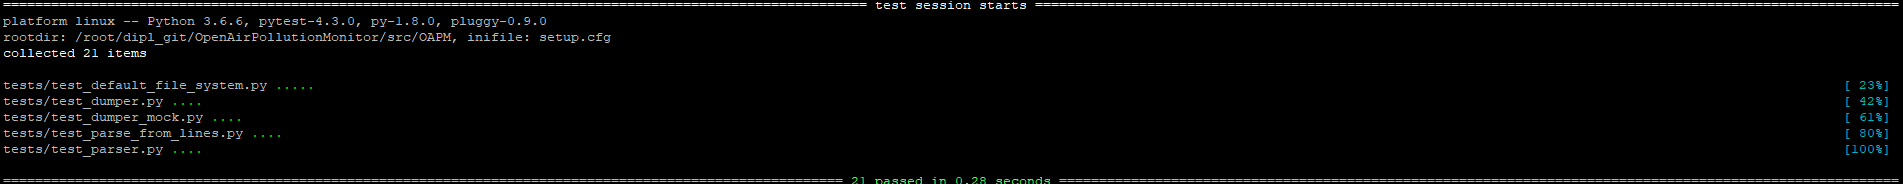
\includegraphics[width=0.7\textwidth]{tests_report}
    \caption{Результаты юнит тестирования}
    \label{pic:lit_testing:tests_report}
\end{figure}
